\documentclass[12pt,xcolor=dvipsnames]{beamer}
\usetheme{CambridgeUS}
\usecolortheme{whale}
\setbeamercolor{block title}{use=structure,fg=white,bg=blue!75!black}  
\setbeamercolor{block body}{use=structure,fg=black,bg=blue!5!white}
\setbeamercolor{frametitle}{bg=Blue}

\usepackage{hyperref}   
\usepackage{url}
\hypersetup{urlcolor=red}

\renewcommand{\bibname}{References}
\setbeamertemplate{bibliography item}{[\theenumiv]}

\usepackage{multicol}
\usepackage{verbatim} 
\usepackage{graphics}
\usepackage{graphicx}


%Basic Information
\title{Data Analytics - Detection of difficulty areas in videos based on student viewing activity}
\author{Arinjoy Basak, Data Analytics group, Mentor: Sukla Nag, Principal investigator: Dr. D. B. Phatak}
\date{\today}

%--------------------------------------------------------------------------------------
%               TITLE PAGE (Slide 1)
%--------------------------------------------------------------------------------------
\begin{document}
\begin{frame}
\titlepage
\end{frame}

%--------------------------------------------------------------------------------------


%--------------------------------------------------------------------------------------
%               Outline
%--------------------------------------------------------------------------------------
%\begin{frame}
%\frametitle{Outline}
%\begin{multicols}{2}
%\tableofcontents[hideallsubsections]
%\end{multicols}
%\end{frame}

%--------------------------------------------------------------------------------------
%               Slide 5
%--------------------------------------------------------------------------------------
\section{Aim and Motivation}
\begin{frame}[t]
\frametitle{A situation}

\begin{itemize}
\item Students watch the videos of a course on a regular basis.
\item They may have difficulty in the videos.
\end{itemize}
This may be due to (among other things)
\begin{itemize}
\item The course videos being difficult for the students to understand
\item The videos not providing sufficient clarity in a subject
\end{itemize}
Result 	
\begin{itemize}
\item i) 	The students do not understand the matter clearly.
\item ii)	They have troubles in assimilating the matter.
\end{itemize}



\end{frame}


%--------------------------------------------------------------------------------------
%               Slide 6
%--------------------------------------------------------------------------------------

\begin{frame}[t]
\frametitle{A situation}

\begin{itemize}
\vspace{70pt}
\item Basically, the instructor would like to know about these things,
\item So that he can understand how his students are responding to his videos - enjoying them or otherwise.
%\item It wouldn't be of much credit if the instructor started giving lessons that were too difficult for the students to understand.
\end{itemize}

\end{frame}


%--------------------------------------------------------------------------------------
%               Slide 7
%--------------------------------------------------------------------------------------
\begin{frame}[t]
\frametitle{Basic outline of the idea}

\begin{itemize}
\item Analyse the student learning behaviour and activities through the events in the lecture videos.
\item The locations of the pauses could be collected as events, and metrics could be developed and appropriate visualizations made to notify or warn the instructors about the difficulty faced by students in particular parts of materials.
\item This could then be met by appropriate measures on the teacher's end, such as

\begin{itemize}
\item Adding more explanatory material
\item Release of an expansion video
\item More quizzes and practice exercises
\item .... and so on.
\end{itemize}

\end{itemize}
\end{frame}


%--------------------------------------------------------------------------------------
%               Slide 8:
%--------------------------------------------------------------------------------------
\section{The Project itself}
\begin{frame}[t]
\frametitle{Steps in the project}

So, given what we aim to achieve through our project, these are the steps we took, one by one:

\begin{itemize}
\item Extracting the data
\item Processing the data
\item Creation and prototyping of the data model
\item Final implementation of the data model
\end{itemize}

\end{frame}

%--------------------------------------------------------------------------------------
%               Slide 9
%--------------------------------------------------------------------------------------
\subsection{Extracting the data}
\begin{frame}[t]
\frametitle{Extracting the data}

\begin{itemize}

\item IITBombayX records the events occurring on the platform as log events in files, spanning gigabytes.

\item Each of the records is a JSON object, having some keys that are common to all events, and some which are dependent on the different events themselves.

\end{itemize}

The following is an example of a log event:

\begin{center}
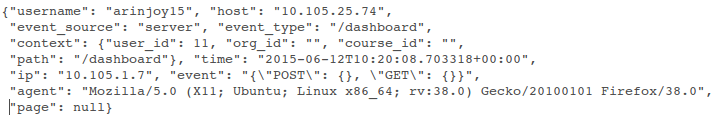
\includegraphics[height=1.8cm]{Diag1.png}\\ % Insert your image it this way
\end{center}

\begin{itemize}
\item These logs were then flattened out, and inserted into a MySQL database. This was the source of data for my project.
\end{itemize}

\end{frame}

%--------------------------------------------------------------------------------------
%               Slide 10
%--------------------------------------------------------------------------------------
\subsection{Processing the data}
\begin{frame}[t]
\frametitle{Processing the data}

In order for us to determine the model on which we were to base our system, we drew our data from the  IITBombayX log files, which were cleaned and made appropriately accessible through MySQL queries, to extract the features that we required. These features included the following:

For a given video:
\begin{itemize}

\item count of the number of times the different regions of the videos were accessed by the different students.
\item total duration spent on the video by the student.

\end{itemize}

\begin{large}
 Our hypotheses: The more number of times a particular region is visited by students, and the longer time students spend there, the more difficult it is for them.
\end{large}

\end{frame}

%--------------------------------------------------------------------------------------
%               Slide 11
%--------------------------------------------------------------------------------------
\begin{frame}[t]
\frametitle{Extracting and Cleaning the required data}

\begin{itemize}
\item A first step involved exploration of the log events and the associated attributes of the logs, to identify the features that we would require to identify each video element for each course, each video event, and to extract the data.

\item At this stage, SQL queries were used to filter and select the relevant data for each video and each user watching it.

\end{itemize}

\end{frame}
%--------------------------------------------------------------------------------------
%               Slide 12
%--------------------------------------------------------------------------------------
\begin{frame}[t]
\frametitle{Extracting and Cleaning the required data}

\begin{itemize}

\item To start with, we first focused our search on videos belonging only to the CS101.1x course (155 videos).

\item To further restrict our search for designing the model, we selected the video with the most number of views, based on the log data, and then selected the user who has accessed that video the most number of times.

\item The end result of this process was a sufficient amount of log data for a single user viewing a single video of a particular course, which would provide enough insight into the patterns of general behaviour of a student or learner.

\end{itemize}

\end{frame}


%--------------------------------------------------------------------------------------
%               Slide 13
%--------------------------------------------------------------------------------------
\begin{frame}[t]
\frametitle{Extracting and Cleaning the required data}

\begin{itemize}

\item The log data also contained repetitions, redundancies and errors.
\item Prior to actual processing, the data extracted from the MySQL table was cleaned further through the Python script written for the prototype.
\item Certain events also had to be reordered and arranged for our purposes in order to make the resultant data more sensible.

\item The development of a complex logic and error checking functions and conditions, and a thorough study of the user events and their sequencing in the logs (and even simulation by self!)

\item Result: a cleaned, chronologically arranged set of events for a particular user


\end{itemize}

\end{frame}


%--------------------------------------------------------------------------------------
%               Slide 8
%--------------------------------------------------------------------------------------
\begin{frame}[t]
\frametitle{MySQL Queries}

At this stage, primarily the data was fetched from MySQL tables for processing, through appropriate queries.

The MysQL tables were:
\begin{itemize}
\item UserSessionOldLog : attributes of interest were userName, moduleSysName, courseName, currVideoSpeed, oldVideoSpeed, createDateTime     (nearly 4 million entries)

\item CourseVideo : attributes of interest were videoSysId, videoUTubeId, videolength (a field we extracted and added later) (1600 entries)

\end{itemize}

\end{frame}

%--------------------------------------------------------------------------------------
%               Slide 8
%--------------------------------------------------------------------------------------
\begin{frame}[t]
\frametitle{MySQL queries}

Some of the queries are as follows:

\begin{itemize}
\item Fetching top 50 most watched videos in CS101.1x

\begin{tiny}
select t.*, CV.videoUTubeId, CV.videolength
	from ( 	
		select moduleSysName, count(eventName) eventCount
		from UserSessionOldLog
		where courseName='CS101.1x' 
			and moduleSysName is not NULL
			and eventType='video'
		group by moduleSysName order by eventCount desc limit 50
		) t,
		(
		select * from CourseVideos where courseName='CS101.1x'
		) CV
	where t.moduleSysName = CV.videoSysName
	order by eventCount desc;
\end{tiny}

\item Highest watched video : videoSysId '67a8559582864d6a8148e2ef5c997e8f'; So, number of viewers in descending order of activity were found as follows:

\begin{tiny}
select userName, count(eventName) watched
	from UserSessionOldLog
	where courseName='CS101.1x' and
		moduleSysName='67a8559582864d6a8148e2ef5c997e8f'
	group by userName order by watched desc limit 10;
\end{tiny}

\end{itemize}

\end{frame}


%--------------------------------------------------------------------------------------
%               Slide 8
%--------------------------------------------------------------------------------------
\begin{frame}[t]
\frametitle{MySQL queries}

\begin{itemize}
\item Finally, for a given user, we found out the distinct events of interest giving us the behaviour of the user in the following manner (say, for the same video as before, but userName='ricky'):

\begin{tiny}
select eventType, eventName, moduleSysName, eventSource, oldVideoTime, currVideoTime, createDateTime from UserSessionOldLog where userName='ricky' and (eventType in ('video') and moduleSysName='67a8559582864d6a8148e2ef5c997e8f' or eventType in ('video', 'navigation') and eventName in ('pageclose', 'saveuserstate') ) order by createDateTime;
\end{tiny}

\end{itemize}

\end{frame}


%--------------------------------------------------------------------------------------
%               Slide 8
%--------------------------------------------------------------------------------------
\begin{frame}[t]
\frametitle{Video length extraction using Google YouTube API}

\begin{itemize}
\item To determine a way to measure the relative amount of time spent by the student on a particular video (such as the fraction of the video playing time)

\item Additional work was done to extract the actual duration of the videos on the all courses using the YouTube id's available for the videos in the CourseVideos table.

\item The Google YouTube API basically sends GET requests online to the API together with the video id and the fields of the 'video' element (a JSON object) that it has to return.

\item We required only the contentDetails attribute of the video element, in which, the value corresponding to the key 'duration' gave us the duration of the video in a ISO 8601 format (PT59M59S), which was processed to make it in seconds.

\end{itemize}

\end{frame}

%--------------------------------------------------------------------------------------
%               Slide 8
%--------------------------------------------------------------------------------------
\begin{frame}[t]
\frametitle{Redundancy removal and Error correction}

\begin{itemize}
\item Removing the redundant data that could be represented by one instance, in order to shorten processing time.
\item This was done programmatically, using complex logic.
\item The following is a simple description of the criteria used to filter out unnecessary data from the results of the query by comparing the rows pairwise, in order of the createDateTime field:


if not (( activity1.eventName == activity2.eventName ) and 	( activity1.oldVideoTime == activity2.oldVideoTime ) and 	( activity1.currVideoTime == activity2.currVideoTime ))

		Then keep the 'activity' in the final list of rows.

else Discard.


\end{itemize}

\end{frame}

%--------------------------------------------------------------------------------------
%               Slide 8
%--------------------------------------------------------------------------------------
\subsection{Creation and prototyping of the data module}
\begin{frame}[t]
\frametitle{Creation and prototyping of the data module}

\begin{itemize}
\item Following the extraction of the data and its cleaning, we had to process the data in order to extract the two features we had proposed earlier.

\item timeFrame : a segment of the video of a certain length (here, we considered 4 seconds)

\item To find the number of accesses to a timeFrame and time duration spent in a timeFrame by a user, given his activities.

\item For this purpose, we considered the type of events we were dealing with: loadvideo, playvideo, pausevideo, seekvideo, stopvideo, saveuserstate, pageclose - and the relation between these events and their sequence of ordering.

\item Inferring actual time spent by the student from the sequence of events, involving tracking whether the video was being played or paused, and when the page was opened or closed.

\end{itemize}

\end{frame}

%--------------------------------------------------------------------------------------
%               Slide 8
%--------------------------------------------------------------------------------------
\begin{frame}[t]
\frametitle{A simplified and ideal sequence of video watching}

\begin{center}
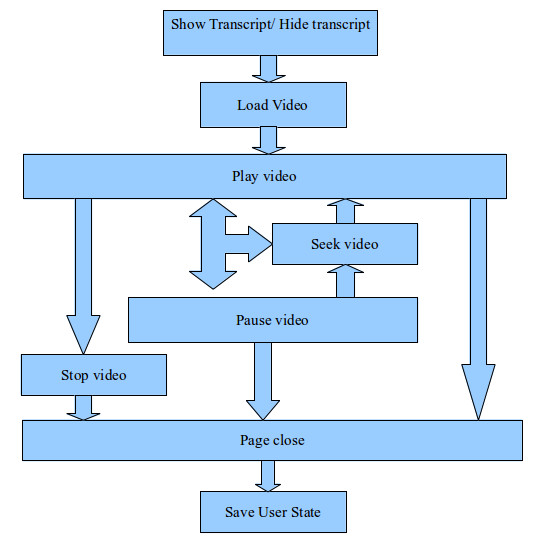
\includegraphics[height=7cm]{Diag3.png}\\ % Insert your image it this way
\end{center}

\end{frame}


%--------------------------------------------------------------------------------------
%               Slide 8
%--------------------------------------------------------------------------------------
\begin{frame}[t]
\frametitle{Creation and prototyping of the data module}

\begin{itemize}

\item The interval between a play and a pause event was considered as the time spent by a student.

\item The time spent upto a seek was considered the time spent by a student, and the seek marking a region that is probably being visited a second time.

\item This stage also involved checking for errors and discrepancies in the data, which was dealt with appropriately to find the proper amount of time spent by a student watching the video.

\item Most of these errors in the timing were probably due to disturbances in the networks, or interleaving of events that is beyond our control at this stage (for example, saveuserstate event always follows pageclose event, but sometimes, it appeared in logs before it - probably due to different ordering in arrival)


\end{itemize}

\end{frame}

%--------------------------------------------------------------------------------------
%               Slide 8
%--------------------------------------------------------------------------------------
\begin{frame}[t]
\frametitle{Creation and prototyping of the data module}

\begin{itemize}
\item The output of this process would be entries of a MySQL table, having a primary key consisting of:\\videoSysId, userName, timeFrameId\\and the attributes frameAccessCount and frameDuration.

\item Finally, we can perform our visualizations, inferences, etc. based on this data.

\item For example, :

\begin{itemize}
\item Total time spent by a user on a particular video
\item Total time spent by all users in a particular timeFrame
\item Total number of accesses to a particular timeFrame
\end{itemize}

which could be made available in the corresponding summary tables as well.
\end{itemize}

\end{frame}

%--------------------------------------------------------------------------------------
%               Slide 8
%--------------------------------------------------------------------------------------
\begin{frame}[t]
\frametitle{An example graph}

The following graph was plotted on the basis of the data obtained by running the module on a single video, and its top 50 users.

\begin{center}
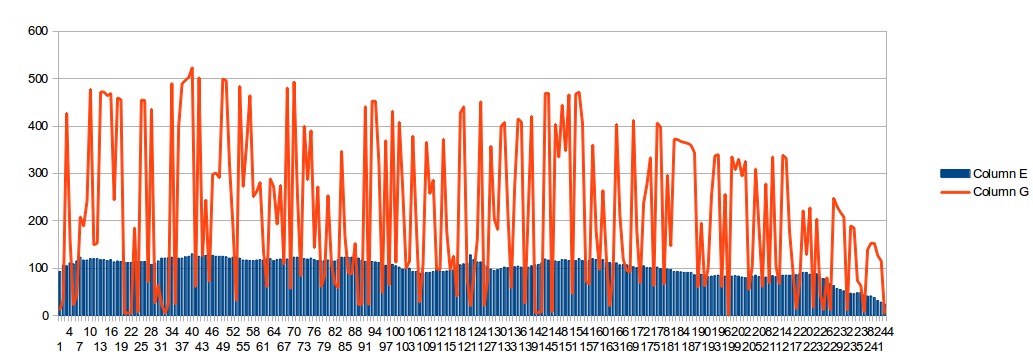
\includegraphics[height=4cm]{Diag2.png}\\ % Insert your image it this way
\end{center}



\begin{tiny}

Legend:X-axis - Time frame number. (dimensionless)
\\Red curve - The total time spent by all the users in a particular timeFrame. (seconds)
\\Blue Columns - The number of accesses to those timeFrames. (dimensionless)\\
\end{tiny}

\end{frame}


%--------------------------------------------------------------------------------------
%               Slide 8
%--------------------------------------------------------------------------------------
\section{Further work in progress}

\begin{frame}[t]
\frametitle{Further work in progress}

The work done so far has been outlined and described. The following are the tasks that are in progress:

\begin{itemize}
\item Spark implementation: The final module would be working in a big data environment - therefore, it needs to be efficient and fast. For this purpose, the final module would be implemented in Spark, and would draw input data from Hive tables through queries and write the result data to hive tables.

\item Further, this data can then be summarized and stored in the corresponding summary tables, which could be accessed during the visualizations provided by the edX Insight module interface provided to the Course Instructor.

\end{itemize}

\end{frame}

%--------------------------------------------------------------------------------------
%               Slide 8
%--------------------------------------------------------------------------------------
\section{Future Work}

\begin{frame}[t]
\frametitle{Future Work}

\begin{itemize}
%\item The data for the individual videos could be clustered to find out the difficult regions in a video, for comparison.

\vspace{70pt}

\item The clustered regions for different videos in a course could be compared with each other in order to find the regions of difficulty, and report them to the instructor.
\end{itemize}

\end{frame}

%--------------------------------------------------------------------------------------
%               Slide 16
%--------------------------------------------------------------------------------------
\section{Technologies Used}
\begin{frame}[t]
\frametitle{Technologies used}

\begin{itemize}

\item MySQL		:	The database management system used

\item Hive		:	The data warehouse infrastructure

\item SparkSQL	:	The fast data processing engine, using in-memory primitives, and faster than Hadoop

\item Python		:	The language base used for programming in this project

\end{itemize}
\end{frame}

%--------------------------------------------------------------------------------------
%               Slide 18:
%--------------------------------------------------------------------------------------

\section{Conclusion}
\begin{frame}[t]
\frametitle{Conclusion}


We wish to extend the edX Insight module to be able to aid the students and instructors in ways both direct and indirect, so that their learning experience is enriched, and the students are able to spend a worthwhile time on the MOOCs they participate in. This project takes a small step in that direction by providing a method for the teachers to find out directly from the activities of the students whether they are facing any difficulty in the videos, without having to communicate with them directly - and ultimately, going towards improvement, and better courses. 

\end{frame}



%--------------------------------------------------------------------------------------
%               Slide 3: Topic 2
%--------------------------------------------------------------------------------------
%\section{Topic 2}
%\begin{frame}[t]
%\frametitle{Topic 2}
%Use the following for creating a table \\
%\begin{center}
%\begin{tabular}{|c|c|c|}
% \hline
% No. & Name & Project \\
% \hline
% 1 & Firuza & Code::Blocks \\
% \hline
% 2 & Birundha & edX \\
% \hline
%\end{tabular}
%\end{center}
%\end{frame}

%---------------------------------------------------------------------------------------
%     Final Slide - References
%--------------------------------------------------------------------------------------
\section{}
\frametitle{}
\begin{frame}[t]

\vspace*{\fill}

\begin{center}
\begin{Huge}THANK YOU\end{Huge}
\end{center}

\vspace*{\fill}

\end{frame}

%---------------------------------------------------------------------------------------
%     Final Slide - References
%--------------------------------------------------------------------------------------
%\section{References}
%\frametitle{References}
%\begin{frame}[allowframebreaks]{References}
%\bibliographystyle{ieeetr}
%\bibliography{biblio}
%\end{frame}
\end{document}




%For bulleted points use the following:\\
%\begin{itemize}
% \item write point 1
% \item write poin 2
%\end{itemize}

%For numbered list use the following:\\
%\begin{enumerate}
% \item write point 1
% \item write point 2
%\end{enumerate}